\documentclass{article}
\pagestyle{empty}
\usepackage{graphicx}
\usepackage{wrapfig}

\newcommand{\inlinecode}[1]{\texttt{#1}}


\begin{document}

\title{Biocellion Command Line Tools}
\date{}
\author{}
\maketitle

\section{\inlinecode{biocellion.py}}

\inlinecode{biocellion.py} runs biological models described with XML using the
biocellion agent based simulation system.  The XML model description file may be
specified directly via the \inlinecode{--xml-file} option, or it make be created
from a template XML file using the \inlinecode{--template-file} option and repeated
use of the \inlinecode{--parm} option.


The tool operates on the model in the following stages:
\begin{wrapfigure}[11ex]{r}{0.4\textwidth}
  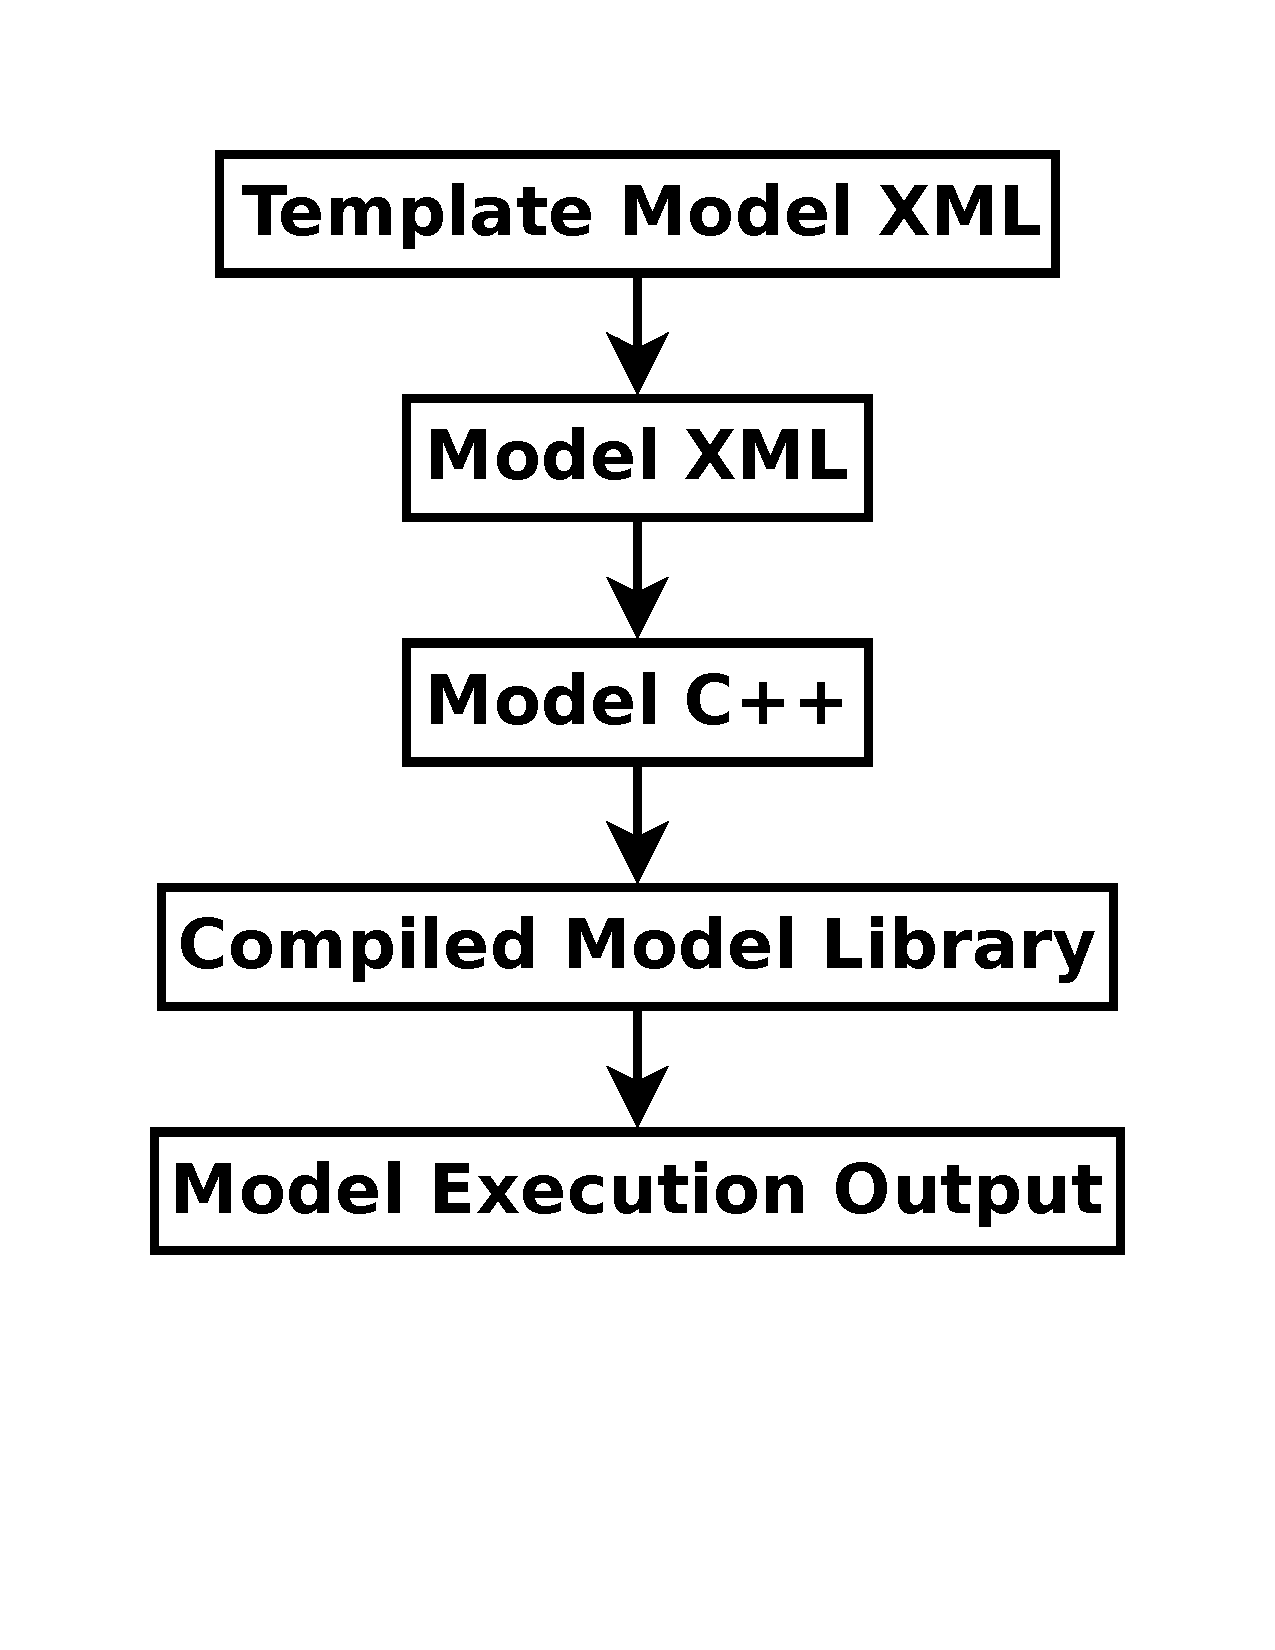
\includegraphics[width=0.38\textwidth]{Stages.pdf}
  \caption{Model processing stages.}
\end{wrapfigure}
\begin{enumerate}
\item Template model XML description file.  This file is an XML model description, with some constants replaced by variables.  The tool will translate the variables into values specified on the command line.
\item Model XML description file.  This is a complete XML model description.
\item Model C++ implementation files.  This is a library of C++ files and auto generated C++ files created from the model XML description file.
\item Model compiled library file.  This is the compiled version of the model C++ files.
\item Model run output data files.  This is the result of running the model using biocellion and the compiled library file.
\end{enumerate}

\subsection{Command Line Options}

Command line options control which of the stages to process and create.


\subsubsection{Stage Processing Commands}

\begin{itemize}
\item \inlinecode{-A | --all-commands}
  process all starting with template xml model file, ending with running model
\item \inlinecode{-T | --process-xml-template}
  process template xml model file into xml model file
\item \inlinecode{-X | --process-xml-model}
  process xml model file into cpp model files
\item \inlinecode{-C | --compile-cpp-model}
  compile cpp model files into model library file
\item \inlinecode{-R | --run-model}
  run the model
\end{itemize}

\subsubsection{XML Options}

\begin{itemize}
\item \inlinecode{-t | --template-file file-name}
  name of input model template XML file
\item \inlinecode{-p | --parm parm=value}
  name and value of parameter for the model; may be specified more than once
\item \inlinecode{-x | --xml-file file-name}
  name of output model XML file
\item \inlinecode{-m | --model-name model-name}
  descriptor for model
\item \inlinecode{-d | --model-dir model-dir}
  location of template and model files
\end{itemize}

Use \inlinecode{-t} and \inlinecode{-x} OR \inlinecode{-m} and \inlinecode{-d}.  Don't mix them.

\subsubsection{Directory and Miscellaneous Options}


\begin{itemize}
\item \inlinecode{-c | --cpp-dir cpp-dir}
  location of cpp model library files.  You should not need to override the default.
\item \inlinecode{-b | --build-dir build-dir}
  directory to create with c++ code
\item \inlinecode{-o | --command-timeout seconds}
  seconds to let the subprocess run the simulation
\item \inlinecode{-h | -? | --help}
  show a help message and quit
\end{itemize}

\subsection{Examples}

\begin{itemize}

\item The following command creates a model instance from the cell-sorting-template.xml, using adhesion values specified on the command line.  It stores the temporary
  model XML file in foo.xml, creates the C++ model in the directory bar, builds and runs the model.  The model is only allowed 180 seconds to execute.

  \inlinecode{bin/biocellion.py --all-commands -t examples/cell-sorting-template.xml -x foo.xml -p RED\_RED\_ADHESION=0.2 -p BLUE\_BLUE\_ADHESION=0.3 -p RED\_BLUE\_ADHESION=0.0 --build-dir bar --command-timeout 180}
  
\end{itemize}


\end{document}
